\documentclass{article}
\usepackage{style}

\begin{document}

\begin{titlepage}
    \begin{center}
        \vspace*{1cm}

        \begin{figure}[H]
        \centering
        
\includegraphics[width=0.25\textwidth]{figures/logos/payload-designer.png}
        \end{figure}
    
        {\Huge\textbf{Payload Designer}}
            
        \bigskip
        \bigskip
        
        {\LARGE A design tool for the FINCH Eye payload}
            
        \bigskip
        \bigskip
        \bigskip
            
        {\Large Software Design Description \\}

        \vfill
        
        {\normalsize Designed and built by \\
        Payload Team \\
        Space Systems Division \\
        University of Toronto Aerospace Team \\}

        \bigskip
        \bigskip
        \bigskip
            
        {\Large \today}

        \begin{figure}[H]
            \centering
            
\includegraphics[trim={0 0 0 0}, clip, width=0.25\textwidth]{figures/logos/utat.png}
            % \caption{}
            \label{fig:logo} 
        \end{figure}
        
    \end{center}
\end{titlepage}







\begin{center}
    \texttt{
    David Maranto,
    Jennifer Zhang,
    Kejsi Gjerazi
    } \\
    University of Toronto
\end{center}


\tableofcontents
\input{\jobname.toc}

\newpage

\section{Introduction}

\section{System}

\section{Specification Definitions}
Definitions for each of the primary payload specifications is provided.

\subsection{Athermal Range}
The athermal range is the temperature range over which the payload is expected to perform without significant degradation in image quality or mechanical stability. It is estimated from the component with the smallest athermalized range, which is essentially the component that is excepted to fail first, should its temperature fall below or rise above its athermal range. See equation \eqref{eq:athermal-range}.

\begin{equation} \label{eq:athermal-range}
    T_{system} = \min_{c \in C} c_{T}
\end{equation}

Where:
\begin{itemize}[label={}]
    \item $T_{system}$: Athermal range of the system.
    \item $C$: Set of all components in the system.
    \item $c_T$: Athermal range of a component.
\end{itemize}

\subsection{Bands}
The bands are the number of spatial or spectral sample points the payload is able to image. 

\subsubsection{Spatial}
The number of spatial bands is related to the number of pixels in the across track direction of the sensor by \eqref{eq:bands-spatial}.

\begin{equation} \label{eq:bands-spatial}
    n_{\text{spatial}} = \frac{ n_{\text{px}_x} }{ n_{\text{bin}_x}}
\end{equation}

Where:
\begin{itemize}[label={}]
    \item $n_{\text{spatial}}$: Number of spatial bands.
    \item $n_{\text{px}_x}$: Number of pixels on the sensor in the across-track direction (see figure \ref{fig:aquisition-methods}).
    \item $n_{\text{bin}_x}$: Number of pixel binning operations.\footnote{Pixel binning is a technique where multiple pixels on a camera sensor are grouped to work together as one.}
\end{itemize}


\subsubsection{Spectral}
The number of spectral bands is the number of samples obtained at the spectral resolution over the target spectral range \eqref{eq:bands-spectral}.

\begin{equation} \label{eq:bands-spectral}
    n_{\text{spectral}} = \frac{\lambda_{\text{max}} - \lambda_{\text{min}}}{\Delta\lambda} 
\end{equation}

Where:
\begin{itemize}[label={}]
    \item $n_{\text{spectral}}$: Number of spectral bands.
    \item $\lambda_{\text{max}}$ [\si{\nm}]: Upper wavelength bound of the spectral range.
    \item $\lambda_{\text{min}}$ [\si{\nm}]: Lower wavelength bound of the spectral range.
    \item $\Delta\lambda$ [\si{\nm}]: Spectral resolution or bandwidth.
\end{itemize}

\subsection{Cost}

\subsection{Field of View}
The field of view is the angular extent that can be imaged by the payload. It can be measured in the along-track or across-track directions \eqref{eq:field-of-view} \cite{specim-fov,wiki-aov,wiki-fov}:

\begin{equation} \label{eq:field-of-view}
\vec{\Phi} = 2\arctan{\left( \frac{\vec{s}}{2f} \right)}
\end{equation}

Where:
\begin{itemize}[label={}]
    \item $\vec{\Phi} = \begin{bmatrix} \Phi_x \\ \Phi_y \end{bmatrix}$ [\si{\degree}]: Fields of view in the across and along track directions.
    \item $\vec{s} = \begin{bmatrix} s_x \\ s_y \end{bmatrix}$ [\si{\mm}]: Slit dimensions in the across and along track directions.
    \item $f$ [\si{\mm}]: Focal length of the foreoptic.
\end{itemize}

\subsection{Instantaneous Field of View}
Instantaneous field of view is the angle subtended by the geometrical projection of single detector element to the target surface. It is given by \eqref{eq:instant-field-of-view} \cite{specim-fov}.

\begin{equation} \label{eq:instant-field-of-view}
\phi = 2\arctan{\left( \frac{d}{2f} \right)}
\end{equation}

Where:
\begin{itemize}[label={}]
    \item $\phi$ [\si{\degree}]: Instantaneous field of view in both the across and along track directions.
    \item $d$ [\si{\micro\m}]: Pixel pitch.
    \item $f$ [\si{\mm}]: Focal length of the foreoptic.
\end{itemize}

Assumes:
\begin{itemize}
    \item Pixels are square. 
\end{itemize}

Field of view

\subsection{Framerate}
The framerate is the frequency at which the sensor core takes images. The max framerate of the payload is given by the hardware limitations of the sensor and any bottlenecks imposed by the payload electronics responsible for collecting the images generated by the sensor, but may not necessarily be the framerate at which images should be taken for the acquisition. 

\subsection{Imaging Orientation}
A 3U cubesat posses two possible imaging orientations. These are: XY and Z. A payload designed to image in the XY imaging configuration would image out of the XY plane. A payload designed to image in the Z imaging configuration would image out of the Z plane. See figure \ref{fig:body-frame}.

\begin{figure}[H]
\centering
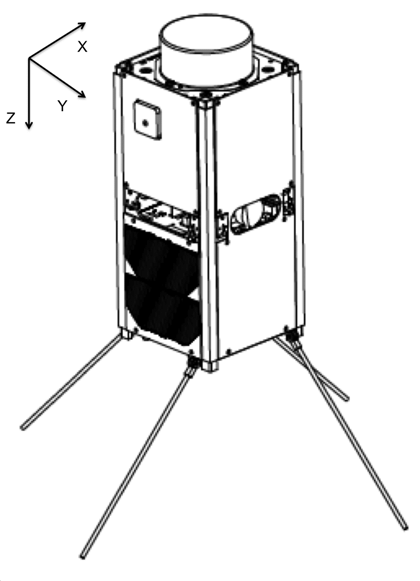
\includegraphics[width=0.5\textwidth]{figures/cubesat-body-frame.png}
\caption{Cubesat body frame definition \cite{CheongEC0}.}
\label{fig:body-frame}
\end{figure}

\subsection{Integrated Cooling}

\subsection{Mass}
The system mass is the net mass of the system.

\begin{equation}
    M_{sys} = \sum_{c \in C} c_M
\end{equation}

Where:
\begin{itemize}[label={}]
    \item $M_{sys}$ [\si{\g}]: Mass.
    \item $c$: Individual component in the system.
    \item $C$: Set of all components in the system.
    \item $c_{M}$ [\si{\g}]: Mass of an individual component.
\end{itemize}

\subsection{Power}

\subsection{Resolution}

\subsubsection{Spatial}
Spatial resolution is given in terms of ground sample distance. In other words, the smallest ground distance resolvable by the payload. The spatial resolution is given by \eqref{eq:spatial-resolution}.

\begin{equation} \label{eq:spatial-resolution}
    \Delta x = \max\left( \Delta x_{\text{sensor}}, \Delta x_{\text{optic}} \right)
\end{equation}

Where:
\begin{itemize}[label={}]
    \item $x_{\text{sensor}}$ [\si{\m}]: Sensor-limited spatial resolution \eqref{eq:spatial-resolution-sensor}.
    \item $x_{\text{optic}}$ [\si{\m}]: Optically-limited spatial resolution \eqref{eq:spatial-resolution-optical}.
\end{itemize}

The sensor-limited spatial resolution is given by \eqref{eq:spatial-resolution-sensor}:

\begin{equation} \label{eq:spatial-resolution-sensor}
    \Delta x_{\text{sensor}} = h \left(\tan{\left(\alpha + \frac{1}{2} \phi \right)} - \tan{\left(\alpha - \frac{1}{2} \phi \right)} \right)
\end{equation}

\todo{fix distinction between slew and skew angle}
\todo{add hyperlinks to variable defined in other sections}
Where:
\begin{itemize}[label={}]
    \item $\Delta x$ [\si{\m}]: Sensor-limited spatial resolution.
    \item $h$ [\si{\km}]: Orbital altitude.
    \item $\alpha$ [\si{\degree}]: Skew angle.
    \item $\phi$ [\si{\degree}]: Instantaneous field of view.
\end{itemize}

Assumes:
\begin{itemize}
    \item Flat Earth. 
\end{itemize}

The optically-limited spatial resolution is given by \eqref{eq:spatial-resolution-optical}.

\begin{equation} \label{eq:spatial-resolution-optical}
    \Delta x_{\text{optic}} = 1.22\frac{\lambda h}{D \cos{\left( \alpha \right)}}
\end{equation}

Where:
\begin{itemize}[label={}]
    \item $\Delta x_{\text{optic}}$ [\si{\m}]: Optically-limited spatial resolution at the center of the field of view.
    \item $\lambda$ [\si{\nm}]: Wavelength of interest.
    \item $h$ [\si{\km}]: Orbital altitude.
    \item $D$ [\si{\mm}]: Aperture diameter.
    \item $\alpha$ [\si{\degree}]: Skew angle.
\end{itemize}


\subsubsection{Spectral}

The sensor-limited spectral resolution is given by \eqref{eq:sensor-limited-spectral-resolution}.

\begin{equation} \label{eq:sensor-limited-spectral-resolution}
    \Delta\lambda_{\text{sensor}} = \frac{\lambda_{\text{max}} - \lambda_{\text{min}} }{ \frac{1}{n_{\text{bin}_{y}}} n_{\text{px}_y} }
\end{equation}

Where:
\begin{itemize}[label={}]
    \item $\Delta x_{\text{sensor}}$ [\si{\m}]: Sensor-limited spatial resolution.
    \item $\lambda_{\text{max}}$ [\si{\nm}]: Upper wavelength bound of the spectral range.
    \item $\lambda_{\text{min}}$ [\si{\nm}]: Lower wavelength bound of the spectral range.
    \item $n_{\text{bin}_{y}}$: Number of pixel binning operations in the along-track direction.
    \item $n_{\text{px}_y}$ [\si{\px}]: Number of pixels in the along-track direction.
\end{itemize}


Spectral resolution is also limited optically by the grating properties. The limit of resolution is determined by the Rayleigh criterion as applied to the diffraction maxima, i.e., two wavelengths are just resolved when the maximum of one lies at the first minimum of the other \cite{grating-resolution}. This resolution is quantified by the grating resolvance \eqref{eq:optically-limited-spectral-resolution}.


\begin{equation} \label{eq:optically-limited-spectral-resolution}
    \Delta\lambda_{\text{optic}} = \frac{\lambda}{R}
\end{equation}

Where:
\begin{itemize}[label={}]
    \item $\lambda$ [\si{\nm}]: Wavelength of interest.
    \item $R$: Resolvance of the grating \eqref{eq:resolvance}.
    \item $\lambda_{\text{min}}$ [\si{\nm}]: Lower wavelength bound of the spectral range.
    \item $\Delta\lambda$ [\si{\nm}]: Spectral resolution or bandwidth.
\end{itemize}

The resolvance is given by \ref{eq:resolvance}:

\begin{equation} \label{eq:resolvance}
    R = mN
\end{equation}

Where:
\begin{itemize}[label={}]
    \item $m$: Order of diffraction.
    \item $N$: Total number of slits illuminated by the incoming beam \eqref{eq:slits-illuminated}.
\end{itemize}

The number of slits illuminated is given by \eqref{eq:slits-illuminated}:

\begin{equation} \label{eq:slits-illuminated}
    N = \nu D
\end{equation}

Where:
\begin{itemize}[label={}]
    \item $\nu$ [\si{\per\mm}]: Line density of the grating.
    \item $D$ [\si{\mm}]: Optical beam diameter of the track.
\end{itemize}

The absolute spectral resolution of the payload is then given by \eqref{eq:spectral-resolution}:

\begin{equation} \label{eq:spectral-resolution}
    \Delta\lambda = \max\left( \Delta\lambda_{\text{sensor}},\Delta\lambda_{\text{optic}} \right)
\end{equation}

Assumes:
\begin{itemize}
    \item No abberations. 
\end{itemize}

\subsubsection{Radiometric}

\subsection{Spectral Range}

\subsection{Swath}
The rectangular ground area the payload sees is referred to as the swath (see figure \ref{fig:swath}).

\begin{figure}[H]
\centering
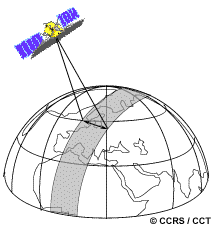
\includegraphics[width=0.5\textwidth]{figures/swath.png}
\caption{Swath width definition \cite{Natural_Resources_Canada2008-bt}.}
\label{fig:swath}
\end{figure}

Swath is calculated by \eqref{eq:swath}.

\begin{equation} \label{eq:swath}
    \vec{S} = h \left(\tan{\left(\vec{\alpha} + \frac{1}{2} \vec{\Phi} \right)} - \tan{\left(\vec{\alpha} - \frac{1}{2} \vec{\Phi} \right)} \right)
\end{equation}

Where:
\begin{itemize}[label={}]
    \item $\vec{S} = \begin{bmatrix} S_x \\ S_y \end{bmatrix}$ [\si{\km}]: Swath dimensions in the across and along track directions.
    \item $h$ [\si{\km}]: Orbital altitude.
    \item $\vec{\alpha} = \begin{bmatrix} \alpha_x \\ \alpha_y \end{bmatrix}$ [\si{\degree}]: Skew angles in the across and along track directions.
    \item $\vec{\Phi} = \begin{bmatrix} \Phi_x \\ \Phi_y \end{bmatrix}$ [\si{\degree}]: Field of views in the across and along track directions. Assumes flat Earth.
\end{itemize}

Assumes:
\begin{itemize}
    \item Flat Earth. 
\end{itemize}

\subsection{Voltage}
The voltage is the voltage required to be supplied to the sensor core.

\subsection{Volume Envelope}
The volume envelope of the payload is the bounding box around the arrangement of the components. The net volume envelope is computed as follows:

\begin{equation}
\vec{V} = \begin{bmatrix} V_x\\ V_y\\ V_z \end{bmatrix} = \begin{bmatrix} \max_{c \in C} c_{V_x}\\ \max_{c \in C} c_{V_y}\\ \sum_{c \in C} c_{V_z} \end{bmatrix}
\end{equation}

Where:
\begin{itemize}[label={}]
    \item $V$ [\si{\cubic\mm}]: Net volume envelope of the payload.
    \item $V_x$, $V_y$, $V_z$ [\si{\cubic\mm}]: Components of the net volume in the $x$, $y$, and $z$ axes of the cubesat reference frame (refer to figure \ref{fig:body-frame}).
    \item $C$: Set of all components in the system.
\end{itemize}

Assumes:
\begin{itemize}
    \item In-line design. 
\end{itemize}

\subsection{Optical Transmittance}
Optical transmittance is the net transmittance for the optical system.

\begin{equation}
    \eta_{optics} = \prod_{c \in C} c_{\eta}
\end{equation}

Where:
\begin{itemize}[label={}]
    \item $\eta_{optics}$: Optical transmittance.
    \item $c$: Individual component in the system.
    \item $C$: Set of all components in the system.
    \item $c_{\eta}$: Optical transmittance of an individual component.
\end{itemize}

\subsection{Signal-to-Noise}
Signal to noise ratio determines how "usable" a signal is after it passes through the optical device. The general formula used to calculate SNR is written as:
\begin{equation}
\text{SNR}(\lambda) = \frac{s(\lambda)_{\text{target}}}{\sigma(\lambda)_{\text{noise}}}
\end{equation} \todo{replace all text in math mode with \\text}
The following sections delve into the assumptions taken and approximations made to arrive at a suitable SNR model for the FINCH eye.

\subsubsection{Signal}

The following derivation assumes the optical system is composed of a single thin lens. We begin by deriving the spectral flux at the aperture of the system. The spectral flux entering the system's aperture is given by \cite{Fiete2001-kz}:

\begin{equation} \label{eq:flux-aperture}
    \Phi_{\text{aperture}}(\lambda) = A_{\text{target}} \cdot \Omega_{\text{aperture}} \cdot L_{\text{target}}(\lambda)
\end{equation}
[\si{\watt\per\meter}]

\todo{Confirm whether Ltarget should be Ltrans times Lrad. Need MODTRAN manual.}

Where:
\begin{itemize}[label={}]
    \item $A_{\text{target}}$ [\si{\meter\squared}]: Area of the ground target.
    \item $L_{\text{target}}(\lambda)$ [\si{\watt\per\steradian\per\meter\squared\per\meter}] (see table \ref{tab:system-params}): Target spectral radiance.
    \item $\Omega$ [degrees?]: Solid angle encompassing the aperture area \eqref{eq:solid-angle} given by \cite{Fiete2001-kz}: \todo{confirm where this comes from}
\end{itemize}

\begin{equation} \label{eq:solid-angle}
    \Omega_{\text{aperture}} = \frac{A_{\text{aperture}}}{R_{\text{target}}^2}  %\steradian
\end{equation}

Where:
\begin{itemize}[label={}]
    \item $A_{\text{aperture}}$ [\si{\meter\squared}]: Area of the system's aperture.
    \item $R_{\text{target}}$ [\si{\meter}]: Distance from the aperture to the ground target.
\end{itemize}

 Substituting \eqref{eq:solid-angle} into \eqref{eq:flux-aperture}:

\begin{equation} \label{eq:flux-aperture-2}
    \Phi_{\text{aperture}}(\lambda) = A_{\text{target}} \cdot \frac{A_{\text{aperture}}}{R_{\text{target}}^2} \cdot L_{\text{target}}(\lambda)
\end{equation}

We wish to express $\Phi_{\text{aperture}}$ in terms of design variables only. To that end, we rewrite $A_{\text{target}}$ in terms of $A_{\text{image}}$ (the image area in \si{\meter\squared}) through the relation \cite{Fiete2001-kz}:

\begin{equation} \label{eq:area-image}
    A_{\text{image}} = m^2 A_{\text{target}}
\end{equation}

Where:
\begin{itemize}[label={}]
    \item $m$: Magnification of the lens, according to the thin lens equation \eqref{eq:snr-magnification}. \cite{Fiete2001-kz}
\end{itemize}

\begin{equation} \label{eq:snr-magnification}
    m = \frac{R_{\text{image}}}{R_{\text{target}}}
\end{equation}

Substituting \eqref{eq:snr-magnification} into \eqref{eq:area-image}:

\begin{equation}
    A_{\text{image}} = \frac{R_{\text{image}}^2}{R_{\text{target}}^2} A_{\text{target}}
\end{equation}

Rearranging for $A_{\text{target}}$:

\begin{equation} \label{eq:area-target}
    A_{\text{target}} = \frac{ R_{\text{target}}^2}{R_{\text{image}}^2} A_{\text{image}}
\end{equation}

We rewrite $R_{\text{image}}$ in terms of the system focal length via the thin lens equation \cite{Fiete2001-kz}:

\begin{equation} \label{eq:snr-thin-lens}
    \frac{1}{R_{\text{target}}} + \frac{1}{R_{\text{image}}} = \frac{1}{f}
\end{equation}

Substituting $R_{\text{target}} = \frac{1}{m}R_{\text{image}}$ (rearranged from \eqref{eq:snr-magnification}) into \eqref{eq:snr-thin-lens} yields:

\begin{equation}
    \frac{m}{R_{\text{image}}} + \frac{1}{R_{\text{image}}} = \frac{1}{f}
\end{equation}

Solving for $R_{\text{image}}$:

\begin{equation}
    R_{\text{image}} = f(m+1)
\end{equation}

The distance of the satellite to the ground target is much greater than the distance of the foreoptic to the image ($R_{\text{target}} \gg R_{\text{image}}$). Therefore, by the thin lens equation:

\begin{equation}
    m \approx 0 \implies R_{\text{image}} \approx f
\end{equation}

Refer to section \ref{sec:thin-magnification} for an explanation of why this is the case.

Substituting $f$ for $R_{\text{image}}$ in \eqref{eq:area-target}:

\begin{equation} \label{eq:area-target-2}
    A_{\text{target}} = \frac{ R_{\text{target}}^2}{f^2} A_{\text{image}}
\end{equation}

Substituting \eqref{eq:area-target-2} into \eqref{eq:flux-aperture-2}:

\begin{equation}
    \Phi_{\text{aperture}}(\lambda) = \frac{R_{\text{target}}^2}{f^2} A_{\text{image}} \cdot \frac{A_{\text{aperture}}}{R_{\text{target}}^2} \cdot L_{\text{target}}(\lambda)
\end{equation}

Simplifying:

\begin{equation}
    \Phi_{\text{aperture}}(\lambda) = A_{\text{image}} \cdot \frac{A_{\text{aperture}}}{f^2} \cdot L_{\text{target}}(\lambda)
\end{equation}

The aperture area $A_{\text{aperture}}$ is given by $\frac{\pi}{4}D^2$ for a circular aperture with diameter $D$ in \si{\meter}. Thus:

\begin{equation}
    \Phi_{\text{aperture}}(\lambda) = A_{\text{image}} \cdot \frac{\pi}{4}\frac{D^2}{f^2} \cdot L_{\text{target}}(\lambda)
\end{equation}

The relation $\frac{D}{f}$ is the inverse of f-number $f_n = \frac{f}{D}$, hence:

\begin{equation} \label{eq:flux-aperture-3}
    \Phi_{\text{aperture}}(\lambda) = A_{\text{image}} \cdot \frac{\pi}{4}\frac{1}{f_n^2} \cdot L_{\text{target}}(\lambda)
\end{equation}

We make use of $f_n$ as a design variable because this quantity is more readily accessible than the aperture diameter $D$\footnote{Body diameter is typically reported on spec sheets for foreoptics, but this is not the same as the aperture diameter. Aperture diameter is smaller than body diameter by the thickness of the shell.}.


The spectral flux reaching the image plane is then given by \cite{Fiete2001-kz}:

\begin{equation}
    \Phi_{\text{image}}(\lambda) = \Phi_{\text{aperture}}(\lambda) \eta_{\text{optics}}
\end{equation}

Where $\eta_{\text{optics}}$ is the transmittance of the optical system (see table \ref{tab:system-params}). Expanding:

\begin{equation}
    \Phi_{\text{image}}(\lambda) = A_{\text{image}} \cdot \frac{\pi}{4}\frac{1}{f_n^2} \cdot \eta_{\text{optics}} \cdot L_{\text{target}}(\lambda)
\end{equation}

The spectral flux on each sensor detector element of the image is given by \cite{Fiete2001-kz}:

\begin{equation}
    \Phi_{\text{detector}} = \frac{A_{\text{detector}}}{A_{\text{image}}} \Phi_{\text{image}}(\lambda) 
\end{equation}

Where $A_{\text{detector}}$ is the area of an individual detector element on the sensor in \si{\meter\squared}. Expanding:

\begin{equation}
    \Phi_{\text{detector}} = \frac{A_{\text{detector}}}{A_{\text{image}}} A_{\text{image}} \cdot \frac{\pi}{4}\frac{1}{f_n^2} \cdot \eta_{\text{optics}} \cdot L_{\text{target}}(\lambda)
\end{equation}

Simplifying:

\begin{equation}
    \Phi_{\text{detector}} = A_{\text{detector}} \cdot \frac{\pi}{4}\frac{1}{f_n^2} \cdot \eta_{\text{optics}} \cdot L_{\text{target}}(\lambda)
\end{equation}

The number of photons $n_\gamma$ reaching the detector element over the integration time\footnote{Integration time is closely related to sensor framerate. It is the time period over which the sensor collects incoming light.} is given by \cite{Fiete2001-kz}:

\begin{equation}
    n_\gamma = \frac{\lambda}{hc} \Delta t \cdot \Phi_{\text{detector}}
\end{equation}

Where:
\begin{itemize}[label={}]
    \item $\lambda$ [\si{\nm}]: Wavelength(s) of interest entering the system (see table \ref{tab:system-params}).
    \item $h$ [\si{\joule\per\hertz}]: Planck's constant.
    \item $c$ [\si{\meter\per\second}]: Speed of light.
    \item $\Delta t$ \si{\second}: Integration time the sensor is configured to use.
\end{itemize}

Expanding:

\begin{equation}
    n_\gamma(\lambda) = \frac{\lambda}{hc} \Delta t \cdot A_{\text{detector}} \cdot \frac{\pi}{4}\frac{1}{f_n^2} \cdot \eta_{\text{optics}} \cdot L_{\text{target}}(\lambda)
\end{equation}


Finally, the signal from the target, measured in electrons generated by the detector element is given by \cite{Fiete2001-kz}:

\todo{might be missing lambda here. Check units}
\begin{equation} 
    s_{\text{target}} = \eta_{\text{sensor}}(\lambda) n_\gamma(\lambda) %\electron
\end{equation}

Where:
\begin{itemize}[label={}]
    \item $\eta_{\text{sensor}}(\lambda)$ [\si{\percent}]: Quantum efficiency of the sensor (see table \ref{tab:system-params}).
\end{itemize}

Expanding:


\begin{equation} 
    s_{\text{target}} = \eta_{\text{sensor}}(\lambda) \cdot \frac{\lambda}{hc} \Delta t \cdot A_{\text{detector}} \cdot \frac{\pi}{4}\frac{1}{f_n^2} \cdot \eta_{\text{optics}} \cdot L_{\text{target}}(\lambda) %\electron
\end{equation}

Rearranging yields:

\begin{equation} 
    \boxed{s_{\text{target}} = \frac{\pi}{4} \frac{\lambda}{hc} \frac{A_{\text{detector}}}{f_n^2} \cdot \eta_{\text{sensor}}(\lambda) \cdot \eta_{\text{optics}}(\lambda) \cdot \epsilon \cdot L_{\text{target}}(\lambda) \Delta t } %electron
\end{equation}

Where:
\begin{itemize}[label={}]
    \item $\epsilon$: Fraction of the light blocked by the slit. It is the slit area divided by the image diameter from the foreoptics incident on the slit face.
\end{itemize}


\footnote{See \href{https://en.wikipedia.org/wiki/Radiance}{radiance}.}

\todo{Confirm modtran accounts for bb radiation in radiance}

\subsubsection{Noise} \todo{units}

Dark noise \cite{noauthor_2019-yu}:

\begin{equation}
    \sigma_{dark} = i_{dark} \Delta t
\end{equation}

Quantization noise \cite{Fiete2001-kz, Wang2019-qd}:

\begin{equation}
    \sigma_{quantization} = \frac{1}{\sqrt{12}} \frac{n_{well}}{2^n_{bit}}
\end{equation}



Net noise \cite{Fiete2001-kz, Chen2012-mt, noauthor_2019-yu}: \todo{Confirm which terms should be squared}

\begin{equation}
    \sigma(\lambda) = \sqrt{ s(\lambda)_{target} + n_{\text{bin}}\sigma_{dark}^2 + \sigma_{quantization}^2 + n_{\text{bin}}\sigma_{read}^2 }
\end{equation}

\todo{implement background signal}

\cite{Chen2012-mt} squares all noise terms, including shot noise. \cite{Fiete2001-kz} squares all terms except shot noise. \cite{noauthor_2019-yu} only squares read noise term. What gives?. Should quantization noise be multiplied by binning operations?


\section{Acquisition Detail Definitions}
Definitions for each of the primary imaging acquisition specifications is provided.

\subsection{Acquisition Framerate}


\subsection{Acquisition Method}
Pushbroom.

\subsection{Datacube Dimensions} \label{sec:datacube-dimensions}
The datacube dimensions specify the shape of the final datacube produced by the sensor in the acquisition. For a perfectly square ground track, the datacube dimensions are given by \eqref{eq:datacube-dimensions}.

\begin{equation} \label{eq:datacube-dimensions}
\vec{F} = \begin{bmatrix} n_{\text{px}_x}\\ n_{\text{px}_x}\\ n_{\text{px}_y} \end{bmatrix}
\end{equation}

Where:
\begin{itemize}[label={}]
    \item $\vec{F}$: Datacube shape.
    \item $n_{\text{px}_x}$ [\si{\px}]: Number of pixels on the sensor in the across-track direction.
    \item $n_{\text{px}_y}$ [\si{\px}]: Number of pixels on the sensor in the along-track direction.
\end{itemize}

\subsection{Datacube size}
The file size of the datacube is given by \eqref{eq:datacube-size}.

\begin{equation} \label{eq:datacube-size}
    F = n_{\text{bit}} \cdot \prod \vec{F}
\end{equation}

Where:
\begin{itemize}[label={}]
    \item $F$ [\si{\mega\byte}]: File size of the datacube. 
    \item $n_{\text{bit}}$ [\si{\bit}]: Bit depth of the sensor.
    \item $\vec{F}$: datacube dimensions \eqref{eq:datacube-dimensions}.
\end{itemize}



\subsection{Duration}
The duration of the acquisition is given by.


\subsection{Ground Track Dimensions}


\subsection{Pointing Accuracy Constraint}
The acquisition's pointing accuracy constraint or tolerance is the maximum allowable deviation from the tracking slew angle that does not result in a smearing of spatial information across the sensor. 

\begin{equation}
    \Delta\theta \leq \arctan\left(\frac{\epsilon \Delta x}{h}\right)
\end{equation}

Where:
\begin{itemize}[label={}]
    \item $h$
\end{itemize} 

Where:
\begin{itemize}[label={}]
    \item $\Delta\theta$ [\si{\degree}]: pointing constraint to satisfy a maximum fractional deviation.
    \item $\epsilon$: Maximum fractional deviation of a ground cell.
    \item $\Delta x$ [\si{\km}]: Ground cell size.
    \item $h$ [\si{\km}]: Orbital altitude.
\end{itemize}

For example, if $\epsilon$ is 0.5, the equation yields a pointing accuracy constraint that ensures a particular ground cell image does not deviate more than half a pixel into a neighbouring pixel from where it should be mapped on the sensor.

\begin{figure}[H]
\centering
\includegraphics[width=0.5\textwidth]{figures/pointing-accuracy-constraint.png}
\caption{Pointing accuracy constraint definition.}
\label{fig:pointing-accuracy-constraint}
\end{figure}

The above equation is derived as follows...

\subsection{Total Acquisition Time}

\begin{equation}
    T = n_{\text{px}_x} \cdot \Delta t
\end{equation}

Where:
\begin{itemize}[label={}]
    \item $T$ [\si{s}]: Total acquisition time.
    \item $n_{\text{px}_x}$: Number of pixels on the sensor in the across track direction (equivalent to the number of scanlines in the acquisition for a square acquisition region).
    \item $\Delta t$ [\si{\ms}]: Integration time of the sensor.
\end{itemize}

As an approximation, $\Delta t$ can be taken to be the inverse of the acquisition framerate \eqref{eq:integration-time}. \todo{can use "..are as previously defined...}

\begin{equation} \label{eq:integration-time}
    \Delta t = \frac{1}{F}
\end{equation}

Where:
\begin{itemize}[label={}]
    \item $\Delta t$ [\si{\ms}]: Sensor integration time.
    \item $F$ [\si{\hertz}]: Sensor framerate.
\end{itemize}

\subsection{Slew Rate}
Slew rate is the rate at which the satellite must rotate in the along-track direction to produce a successful acquisition without the swath moving too fast such that the acquisition misses parts of the terrain, or too slow such that parts of the terrain double up in the acquisition.


\begin{equation} \label{eq:slew-rate}
    \dot{\theta} = \arctan{\frac{1}{h}\left( v_{\text{ground}} - v_{\text{ground,required}} \right)}
\end{equation}

Where:
\begin{itemize}[label={}]
    \item $\dot{\theta}$ [\si{\degree\per\s}]: Slew rate.
    \item $h$ [\si{\km}]: Orbital altitude.
    $v_{\text{ground}}$ [\si{\m\per\s}]: \eqref{eq:velocity-ground} Ground-projected orbital velocity.
    \item $v_{\text{ground,required}}$ [\si{\m\per\s}]: \eqref{eq:velocity-ground-required} Required ground-projected orbital velocity to ensure each ground swath is correctly acquired.
\end{itemize}

\begin{equation} \label{eq:velocity-ground-required}
    v_{\text{ground,required}} = \frac{S_x}{T} 
\end{equation}
Where $v_{\text{ground,required}}$ [\si{\m\per\s}] is the required ground-projected orbital velocity to ensure each ground swath is correctly acquired.


\section{Component Spacing Modelling}

\section{Component Specifications}

\subsection{Foreoptics}
The fore-optics of the spectrometer is the entrance optics, which serves as a telescope. Although its components are unknown, it can be treated as a black box.

\begin{figure}[H]
\centering
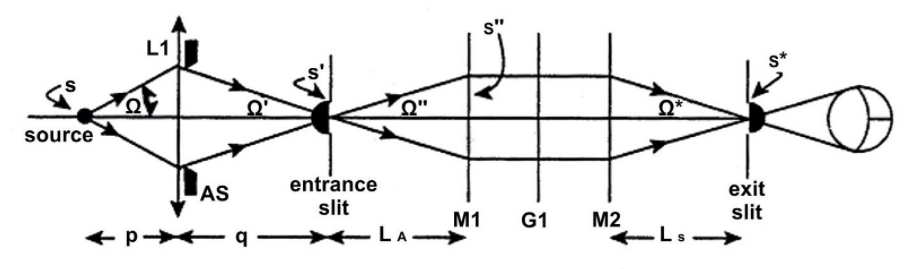
\includegraphics[width=1\textwidth]{figures/monochromator.PNG}
\caption{A monochromator system. \cite{Horiba_throughput_etendue}}
\label{fig:monochromator}
\end{figure}

\subsubsection{Aperture Diameter}
The aperture diameter of the foreoptics is the diamter of the foreoptic lens, and can be calculated by rearranging equation \ref{eq:f-num}. Note: When the object distance is very far (approaches infinity), the image distance is effectively the same as the focal length of the lens.

\begin{equation} \label{eq:aperture-diameter}
    d=\frac{q}{f/value}=2q\times NA
\end{equation}

Where:
\begin{itemize}[label={}]
    \item $NA$: Numerical aperture.
    \item $q$ [\si{\mm}]: Image distance from the foreoptic lens.
    \item $f/value$: f/number of the foreoptic system.
\end{itemize}

\subsubsection{Effective Focal Length}
Effective Focal Length (EFL) is the distance from a principal plane of an optical lens to its imaging plane. The principle plane is a hypothetical plane where incident light rays can be considered to bend due to refraction, and the imaging plane is where the image is formed\cite{Edmund_lens_geometries}.

EFL is calculated using the thin lens equation \ref{eq:thin-lens}, as the image distance.

\subsubsection{Telecentricity}
*Add*

\subsubsection{Magnification}
The magnification of the foreoptics is the ratio of the image and object distances. \cite{Horiba_entrance_optics}:

\begin{equation} \label{eq:foreoptics-magnification}
    M = \frac{q}{p}
\end{equation}

Where:
\begin{itemize}
    \item $M$: Magnification.
    \item $q$: Image distance from foreoptic lens.
    \item $p$: Object distance from foreoptic lens.
\end{itemize}
Refer to Figure \ref{fig:monochromator}.

\subsubsection{Numerical Aperture}
The numerical aperture is the light gathering power of an optic, characterizing the range of angles of light rays that can enter or exit an optical component (e.g. lens, slit) \cite{Horiba_monochromator}.

\begin{equation} \label{eq:numerical-aperture}
    NA = \mu\sin\Omega
\end{equation}

Where:
\begin{itemize}[label={}]
    \item $\mu$: Refractive index (1 in air).
    \item $\Omega$ [\si{\degree}]: Angle of the marginal ray from the optical axis
\end{itemize}
Refer to Figure \ref{fig:monochromator}.

``The numerical aperture (1/f-number/2) sets the angle of the rays at the edge of the focused cone of energy. This must be tied in with the maximum AOI at the edge of the field (acceptable deviation from perfect telecentricity). This should be considered when determining the first order specifications." ---Tymen Nagel from Chromar Technologies

\subsubsection{Back Focal Length}
Back focal length (BFL) is defined as the distance from the backmost mechanical plane of the fore-optics to the focal plane, where the slit is mounted. This is thus a purely mechanical constraint, and consultation with the Payload Structures team is warranted. The \texttt{program} will not include BFL as an optical parameter.

\subsubsection{F/number}
The F/number, often known as the F value, of a lens system is the ratio of the image distance to the diameter of the slit. The f/number is usually set by adjusting the diaphragm/aperture in most lens systems. The lower the lens’ f/number, the larger the iris, and more light is able to pass through the system (greater throughput). The f/number usually increases by multiple of $\sqrt{2}$, since the aperture area typically varies by a factor of 2 \cite{Hollows_undated}.

\begin{equation} \label{eq:f-num}
    fnum = \frac{1}{2NA} = \frac{q}{d}
\end{equation}

Where:
\begin{itemize}[label={}]
    \item $NA$: Numerical aperture.
    \item $q$ [\si{\mm}]: Image distance from the foreoptic lens.
    \item $d$ [\si{\mm}]: Diameter of the aperture in the foreoptic system.
\end{itemize}
Note: When the object distance is very far (approaches infinity), the image distance is effectively the same as the focal length of the lens.
Note: $NA = sin(\Omega)$, from Figure \ref{fig:monochromator}, which approximates to $\frac{1}{2f/number}$ \cite{Horiba_monochromator}.

\subsubsection{Geometric Etendue}
The geometric etendue of an optical system is its ability to accept light, characterized by the maximum beam size the optical component can accept. As such, it can limit light throughput of the spectrometer. It is calculated by \cite{Horiba_throughput_etendue}:

\begin{equation} \label{eq:geometric-etendue}
    G = \pi\Sigma\sin^2\Omega
\end{equation}

Where:
\begin{itemize}[label={}]
    \item $G$: Geometric etendue.
    \item $\Omega$ [\si{\degree}]: Angle of the marginal ray from the optical axis.
\end{itemize}

\subsubsection{Flux}
From the geometric etendue, flux, defined as “energy/time (photons/sec, or watts) emitted from a light source or slit of given area, into a solid angle at a given wavelength (or bandpass)”, can be calculated \cite{Horiba_throughput_etendue}:

\begin{equation} \label{eq:flux}
    \phi = B\times G
\end{equation}

\begin{equation} \label{eq:flux-expanded}
    \phi = B\pi S'\sin^2\Omega'
\end{equation}

Where:
\begin{itemize}[label={}]
    \item $\phi$ [\si{\watt}]: Flux.
    \item $B$ [\si{\watt\per\steradian\mm\squared}]: Radiance of the source.
    \item $S'$ [\si{\mm\squared}]: Area of the entrance slit or emitting source.
    \item $\Omega$ [\si{\degree}]: Angle of the marginal ray from the optical axis, shown in Figure \ref{fig:monochromator}.
\end{itemize}

\subsection{Slit}
\begin{figure}[H]
\centering
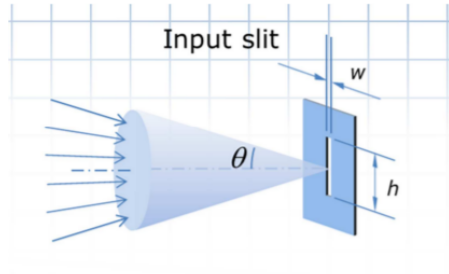
\includegraphics[width=0.6\textwidth]{figures/entrance slit.PNG}
\caption{Light arriving at the entrance slit of a spectrometer. \cite{Ibsen_photonics_coupling}}
\label{fig:entrance-slit}
\end{figure}

The light output from the fore-optics passes through a narrow slit, which plays a large role in determining the throughput of the optical system (i.e. amount of light, measured by photon flux) and resolution. These are affected by the size (length and width) of the entrance slit; slit length in the horizontal direction and slit width in the vertical. In figure \ref{fig:entrance-slit}, which shows the slit sideways, $h$ is the length and $w$ is the width. The standard slit length is 1 mm, with options of up to 2 mm available as well \cite{B&W_Tek}; since the spectrometer should have a magnification of 1, the slit length should equal the detector width. Slit widths range from 5$\mu m$ to 800$\mu m$, with standard sizes: 10, 14, 25, 50, 100 and 200 $\mu m$ \cite{StellarNet}. It must be placed exactly within the optical path of the spectrometer, its distance from the fore-optics dependent on the image distance from the fore-optic lens \cite{Horiba_entrance_optics}, and distance from the collimator dependent on the focal point of the collimation lens \cite{Ibsen_photonics_design}.

Decreasing the slit width blocks incoming light travelling at larger angles, with respect to the optical axis, improving resolution while decreasing light throughput. Therefore, both factors must be taken into consideration when optimizing slit width \cite{Optecks}.

\subsection{Lens}
The lens models we derive here apply for lenses operating on light which is collimated\footnote{\href{https://en.wikipedia.org/wiki/Collimated_beam}{Collimated light} is light whose rays propagate in parallel.} either on the onset or outset. We focus on these two scenarios because the payload specifically makes use of lenses acting as either \textit{collimators} or \textit{focusers}. A collimator takes a point source of light (i.e. light exiting the slit) and produces a collimated beam. A focuser takes collimated light and produces an image (i.e. the lens responsible for focusing the diffracted light from the diffractor onto the sensor). Despite being a distinguishing factor between candidate models, chromatic aberrations are not taken into account for the reasons noted in section \ref{sec:scope}.

\begin{figure}[H]
    \centering
    \subfloat[\centering Collimator]{{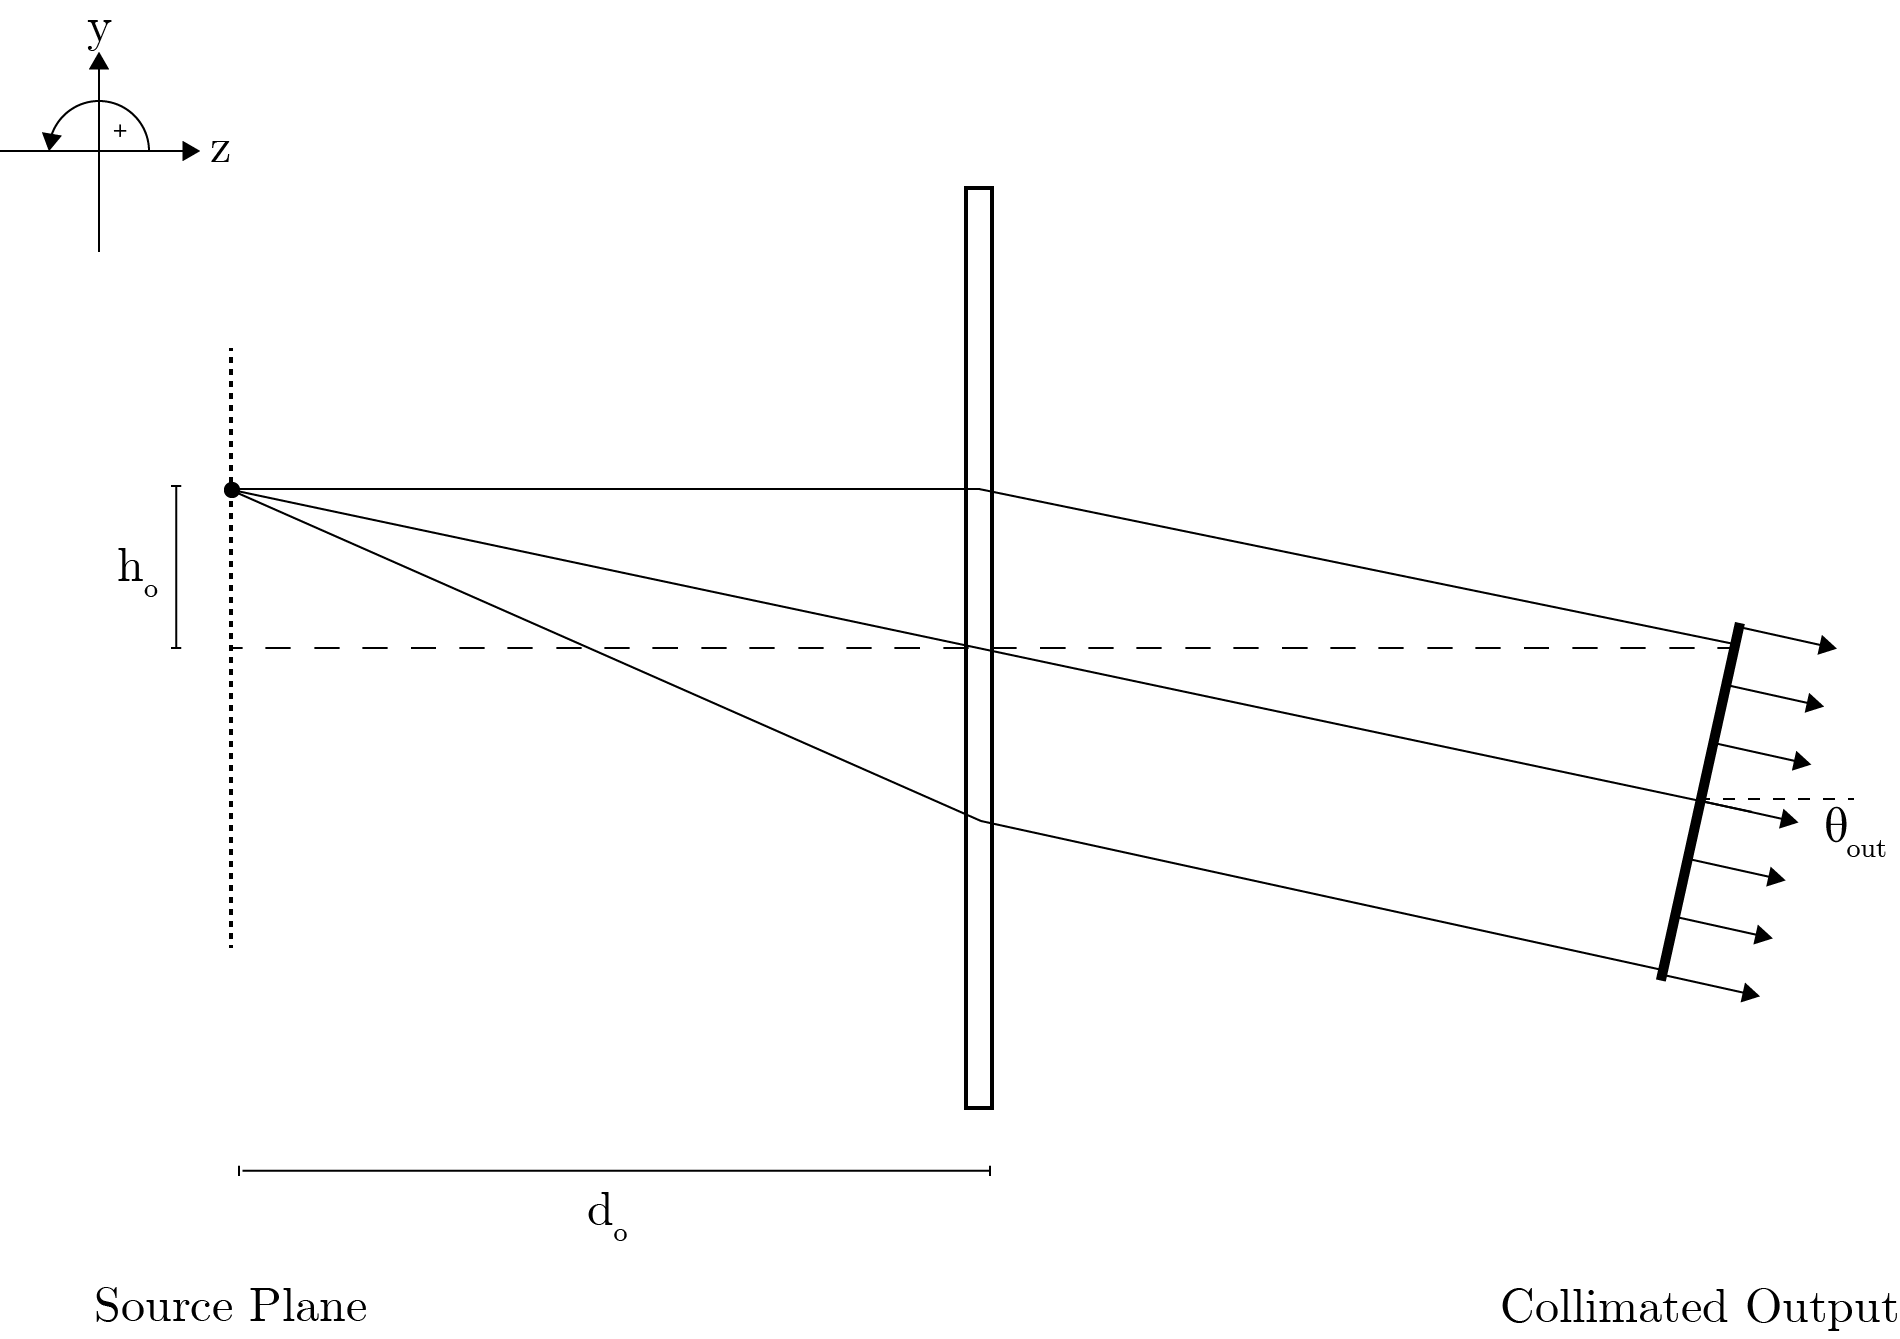
\includegraphics[width=0.45\textwidth]{figures/thin-collimator-model.png}}}
    \qquad
    \subfloat[\centering Focuser]{{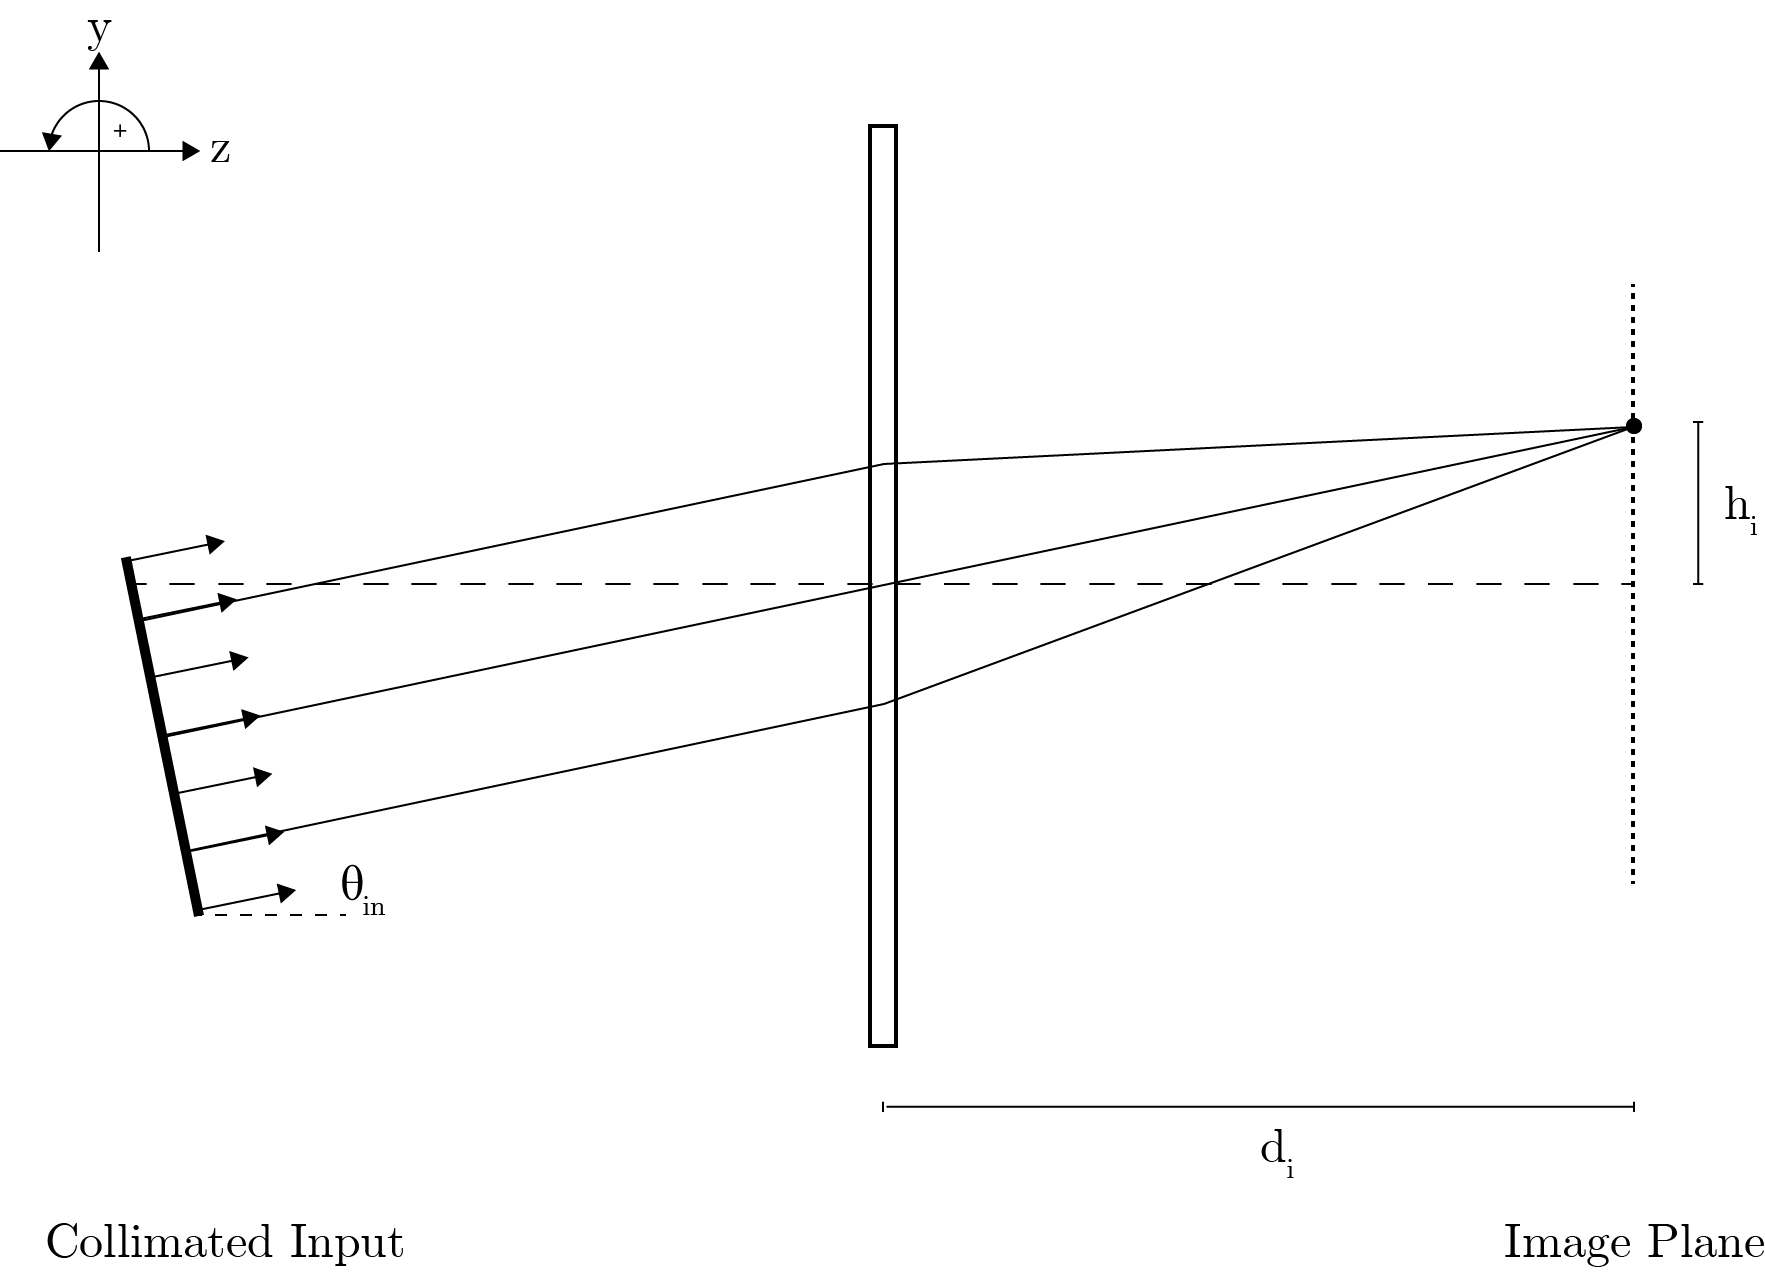
\includegraphics[width=0.45\textwidth]{figures/thin-focuser-model.png}}}  
    \caption{Thin singlet models.}
    \label{fig:thin-singlet-lens-models}
\end{figure}

\subsubsection{Thin Singlet Lens Model} \label{sec:thin-singlet-model}

A thin lens is a mathematical approximation of a real lens. For sufficiently thin lenses, the thin lens equations are an adequate description of the characteristics of the lens \cite{Boundless_undated-to}.

Assumptions:
\begin{itemize}
    \item Rays are paraxial.\footnote{Paraxial rays are rays of light at small enough angles from the optical axis that they are well described by the small angle approximation \cite{noauthor_undated-wt}.} 
    
    \item Lens is of negligible thickness.
    
    \item Incoming light to the focuser or outgoing light from the collimator is perfectly collimated.
    
    \item Does not account for field curvature.\footnote{\href{https://en.wikipedia.org/wiki/Petzval_field_curvature}{Field curvature} is a type of optical aberrations in which a flat object normal to the optical axis cannot be brought properly into focus on a flat image plane, but instead the focal plane ends up curved.}
\end{itemize}

\subsubsection{Source \& Image Distances} \label{sec:thin-object-image-distances}
The source distance of a thin lens is the distance between a point source of light and the lens. The image distance is the distance between the lens and the image plane. This distance is approximated by the thin lens equation \cite{noauthor_undated-zn}:

\begin{equation} \label{eq:thin-lens}
    \frac{1}{f} = \frac{1}{d_o} + \frac{1}{d_i}
\end{equation}

Where:
\begin{itemize}[label={}]
    \item $f$: Focal length of the thin lens.
    \item $d_o$ [\si{\mm}]: Distance from the source to the lens.
    \item $d_i$ [\si{\mm}]: Distance from the lens to the image.
\end{itemize}

\begin{enumerate}
    \item In the case of a thin focuser, input rays are parallel, and may be represented by a source that is an infinite distance away. Output rays converge, hence the image is at a finite distance after the lens. Thus:
    
    \begin{equation} \label{eq:image-distance}
        {d_i = f}    
    \end{equation}
    
    \item In the case of a thin collimator, incoming rays diverge, hence the source is at a finite distance before the lens. Outgoing rays are collimated, which may be represented by an image at an infinite distance away. Thus:
    
    \begin{equation} \label{eq:source-distance}
        {d_o = f}
    \end{equation}
\end{enumerate}

\subsection{Dichroic Bandpass Filter Model}

A Dichroic Bandpass Filter uses dielectric layers on glass that transmit a desired range of wavelengths, and reflects the rest. These filters can be categorized into single-cavity and multi-cavity, based on the model.

\begin{figure}[H]
    \centering
    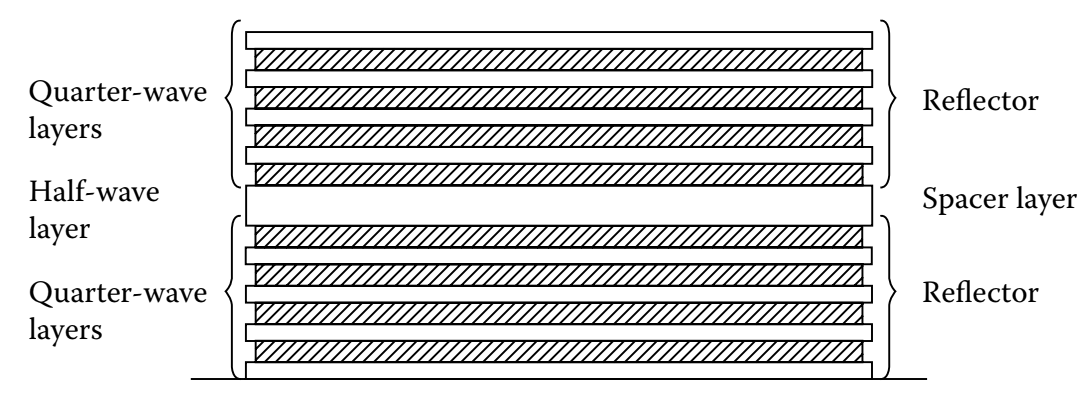
\includegraphics[width=0.7\textwidth]{figures/Single_Layer_Dichroic.png}
    \caption{Single Cavity Dichroic Bandpass Filter}
    \label{fig:my_label}
\end{figure}

\subsubsection{Phase Shift}
The phase shift of a non-normal incident beam is represented by the following equation:

\begin{equation} \label{eq:phase-shift}
    \lambda_\theta = \lambda_0 \times \sqrt{1 - \left( \frac{n_0}{n^*} \sin\theta \right)^2}
\end{equation}

Where:
\begin{itemize}[label={}]
    \item $\lambda_\theta$ [\si{\nm}]: Wavelength of the beam at angle of incidence $\theta$.
    \item $\lambda_0$ [\si{\nm}]: Wavelength of the beam at normal incident angle.
    \item $n_0$: Refractive index of incident medium.
    \item $n^*$: Effective refractive index of the bandpass filter.
\end{itemize}

Note: Although the filter is made of multiple layers with different indices of refraction, phase shift calculations of the entire system can be done using the effective refractive index, which has a value that is between the highest and lowest indices of the filter layers.

\subsubsection{Reflected Beam}
According to Cushing, the reflectances from a dichroic bandpass filter is expressed by the following equation:

\begin{equation} \label{eq:reflected-beam}
    \sqrt R = \frac{n^* - n_0}{n^* + n_0}
\end{equation}

Where:
\begin{itemize}[label={}]
    \item $n_0$: Refractive index of the incident medium.
    \item $n^*$: Effective refractive index of the filter.
\end{itemize}

%Kejsi 
\subsection{VPH Grism Model} \todo{units}

\begin{figure}[H]
\centering
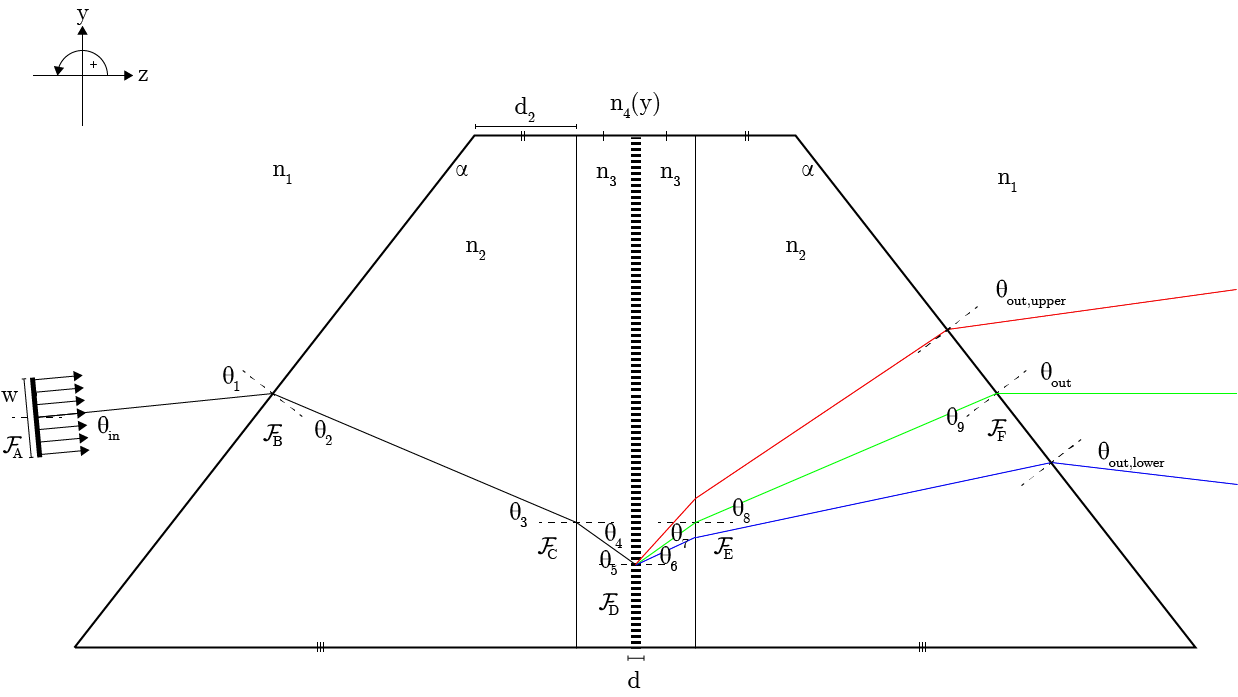
\includegraphics[width=\textwidth]{figures/grism-model.png}
\caption{The VPH grism model diagram.}
\label{fig:grism-model}
\end{figure}

\subsubsection{Angular distribution of diffracted wavelengths}
Snell's law and the grating equation are applied on a bundle of collimated light entering the grism at some angle $\theta_{in}$. The angular distribution of diffracted wavelengths is a mapping between the wavelengths produced by the diffractor and the angles at which those wavelengths leave the component. The first angle from figure \ref{fig:grism-model} is given by:
\begin{equation}
\theta_1 = \theta_{in} + \alpha
\end{equation}

Where:
\begin{itemize}[label={}]
    \item $\alpha$ is the apex angle of the prisms
    \item $\theta_{in}$ is the 
\end{itemize}
The second angle in figure \ref{fig:grism-model} is given by using Snell's Law \cite{Wikipedia_contributors_undated-ti}:
\begin{align} 
\theta_2 &= \arcsin\left( \frac{n_1}{n_2} \sin\left( \theta_1 \right) \right) 
\end{align} 
Where:
\begin{itemize}[label={}]
    \item $n_1$ is index of refraction of the external medium prism medium
    \item $n_2$ is index of refraction of the prism medium
    \item $\theta_1$ is the previously calculated angle
\end{itemize}

The next three angles are:
\begin{equation}
\theta_3 = \alpha - \theta_2
\end{equation}

\begin{equation}
\theta_4 = \arcsin\left( \frac{n_2}{n_3} \sin\left( \theta_3 \right) \right) 
\end{equation}
Where:
\begin{itemize}[label={}]
    \item $n_3$ is the index of refraction of the VPH hermetic seal medium
\end{itemize}

\begin{equation}
\theta_5 = \theta_4
\end{equation}

The sixth angle is found with the grating equation and is wavelength specific because at this point in the grism the light has been dispersed \cite{Barden1999-vq, Barden2000-sv}: 
\begin{align} 
\theta_6 &= \arcsin\left( \sin\left( \theta_5 \right) - m\nu\lambda \right)
\end{align}
Where:
\begin{itemize}[label={}]
    \item $m$ is the order of diffraction
    \item $\nu$ is the grating frequency
    \item $\lambda$ is the wavelength of light of interest
\end{itemize}

\begin{equation}
\theta_7 = \theta_6
\end{equation}

\begin{equation}
\theta_8 = \arcsin\left( \frac{n_3}{n_2} \sin\left( \theta_7 \right) \right) 
\end{equation}

\begin{equation}
\theta_9 = \theta_8 - \alpha
\end{equation}

\begin{equation}
\theta_{10} = \arcsin\left( \frac{n_2}{n_1} \sin\left( \theta_9 \right) \right)
\end{equation}

The final exit angle of the light at the desired wavelength is then found with:
\begin{equation}
\boxed{\theta_{out} = \theta_{10} + \alpha}
\end{equation}

\subsubsection{Undeviated Wavelength}
The undeviated wavelength is the wavelength which exits the grating at an angle equal and opposite to the angle of incidence with respect to the grating surface normal. The undeviated wavelength is given by:
\begin{align}
\lambda_g &= 2 \frac{\sin\left( \alpha \right)}{m\nu}
\end{align}
Where:
\begin{itemize}[label={}]
    \item $\alpha$ is the angle of incidence
    \item $m$ is the order of diffraction
    \item $\nu$ is the grating frequency
\end{itemize}

\subsubsection{Diffraction Efficiency}
The diffraction efficiency of a grism is the proportion of light that will be transmitted at the exit of the component. It is found with:

\begin{equation}
\eta = T_p^2\left(sin^{2}\left(\frac{\pi \Delta n_g d}{\lambda \cos{\left(\alpha_{g}\right)}}\right) + \frac{1}{2} \sin^{2}\left[\frac{\pi \Delta n_g d}{\lambda \cos{\left(\alpha_{g}\right)}} \cos(2 \alpha_{g})\right]\right)
\end{equation}
Where: 
\begin{itemize}[label={}]
    \item $\eta$ is the diffraction efficiency with respect to the plane of incidence.
    \item $\Delta n_g$ is the index modulation contrast.
    \item $d$ is the grating thickness.
    \item $\alpha_g$ is the angle of incidence.
    \item $T_p$ is the transmittance of the prism medium.

This equation holds for this condition:
\begin{equation}
Q = \frac{2\pi\lambda d}{n_g \Lambda^2} > 10
\end{equation}
Where:
\begin{itemize}[label={}]
    \item $\Lambda$ is $\frac{1}{\nu_g}$, $\nu_g$ being the fringe frequency.
\end{itemize}

\subsubsection{Resolvance}
Resolvance or resolving power is a common way of expressing resolution for a grating, which is a measure of the grating's ability to separate two wavelengths. Resolvance is found with: 
\begin{equation}
R = \frac{\lambda}{\Delta \lambda} = mN
\end{equation}

Where:
\begin{itemize}[label={}]
    \item $\lambda$ is the wavelength of interest.
    \item $\Delta \lambda$ is the resolution.
    \item $m$ is the diffraction order.
    \item $N$ is the number of grooves in the grating. 
\end{itemize},  and  \cite{Hyperphysics}. 

\section{Orbital Parameters}

\subsection{Orbital Velocity}
Orbital velocity \eqref{eq:velocity-orbit} is a measure of how quickly the satellite moves along the trajectory of its orbit. This is not a vector quantity, so technically this is orbital speed.

\begin{equation} \label{eq:velocity-orbit}
    v_{\text{orbit}} = \sqrt{\frac{\mu_E}{R_{\text{orbit}}}}
\end{equation}

Where:
\begin{itemize}[label={}]
    \item $v_{\text{orbit}}$ [\si{\km\per\s}]: The orbital velocity of the satellite.
    \item $\mu_E$ [\si{\m\cubed\per\s\squared}]: Geocentric gravitational constant (table \ref{tab:constants}).
    \item $R_{\text{orbit}}$ [\si{\km}]: Orbital radius of the satellite \eqref{eq:orbit-radius}.
\end{itemize}

\subsection{Ground-Projected Orbital Velocity}
The ground-projected orbital velocity \eqref{eq:velocity-ground} can be thought of as the velocity of the shadow the satellite casts along the ground if the sun was directly above it.

\begin{equation} \label{eq:velocity-ground}
    v_{\text{ground}} = \omega_{\text{orbit}} R_E
\end{equation}

Where:
\begin{itemize}[label={}]
    \item $v_{\text{ground}}$ [\si{\km\per\s}]: The ground-projected orbital velocity of the satellite.
    \item $\omega_{\text{orbit}}$ [\si{\degree\per\s}]: angular velocity of the satellite in orbit with respect to the Earth's center \eqref{eq:velocity-orbit-angluar}.
    \item $R_E$ [\si{\km}]: Radius of Earth (table \ref{tab:constants}).
\end{itemize}

\subsection{Orbital Angular Velocity}
Orbital angular velocity refers to how fast a point object revolves about a fixed origin. In other words, the time rate of change of its angular position relative to the center of the Earth. It is given by \eqref{eq:velocity-orbit-angluar}.

\begin{equation} \label{eq:velocity-orbit-angluar}
    \omega_{\text{orbit}} = \frac{v_{\text{orbit}}}{R_{\text{orbit}}}
\end{equation}

Where:
\begin{itemize}[label={}]
    \item $\omega_{\text{orbit}}$ [\si{\degree\per\s}]: The angular velocity of the satellite.
    \item $v_{\text{orbit}}$ [\si{\m\per\s}]: The satellite's orbital velocity \eqref{eq:velocity-orbit}.
    \item $R_{\text{orbit}}$ [\si{\km}]: The satellite's orbital radius measured from the Earth's center \eqref{eq:orbit-radius}.
\end{itemize}


\subsection{Orbital Radius}
The orbital radius is the distance between the satellite in orbit and the center of the Earth. It is given by \eqref{eq:orbit-radius}.

\begin{equation} \label{eq:orbit-radius}
    R_{\text{orbit}} = R_E + h
\end{equation}

Where:
\begin{itemize}[label={}]
    \item $R_{\text{orbit}}$ [\si{\km}]: The satellite's orbital radius.
    \item $R_E$ [\si{\km}]: Radius of the Earth (table \ref{tab:constants}).
    \item $h$ [\si{\km}]: The satellite's orbital altitude.
\end{itemize}

\end{itemize}
\printbibliography

\appendix
\appendixpage

\section{Derivations}



\subsection{Geometric Etendue}
Geometric etendue is calculated by \cite{Horiba_throughput_etendue}:

\begin{equation}
    d^2G = \frac{dS}{dQ}
\end{equation}

\begin{equation}
    G = \iint\frac{dS}{dQ}
\end{equation}

Where:
\begin{itemize}[label={}]
    \item $G$ [units]: Geometric etendue.
    \item $S$ [units]: Area of the emitting source.
    \item $Q$ [units]: Solid angle into which light propagates (2$\Omega$ in Figure \ref{fig:monochromator}).
\end{itemize}

Through integration:

\begin{equation}
    G = \pi\Sigma\sin^2\Omega
\end{equation}

Where:
\begin{itemize}[label={}]
    \item $G$ [units]: Geometric etendue.
    \item $\Omega$ [units]: Angle of the marginal ray from the optical axis.
\end{itemize}

\subsection{Source \& Image Distances}
\begin{enumerate}[(a)]
    \item In the case of a thin focuser, input rays are parallel, and may be represented by a source that is an infinite distance away. Output rays converge, hence the image is at a finite distance after the lens. Thus:
    \begin{equation}
        \frac{1}{f} = \lim_{d_o\to\infty} \frac{1}{d_o} + \frac{1}{d_i} = \frac{1}{d_i}
    \end{equation}
    
    \begin{equation} \label{eq:image-distance}
        \Rightarrow \ \boxed{d_i = f}    
    \end{equation}
    
    \item In the case of a thin collimator, incoming rays diverge, hence the source is at a finite distance before the lens. Outgoing rays are collimated, which may be represented by an image at an infinite distance away. Thus:
    \begin{equation}
        \frac{1}{f} = \lim_{d_i\to\infty} \frac{1}{d_o} + \frac{1}{d_i} = \frac{1}{d_o}
    \end{equation}
    
    \begin{equation} \label{eq:source-distance}
        \Rightarrow \ \boxed{d_o = f}
    \end{equation}
\end{enumerate}

\subsection{First-Order Model: Thin Lenses in Contact} - move to appendix
\todo{Note: these are Shiqi's derivations. Should be ok but would be good to find source.}

The simplest model assumes lenses are thin and in contact.

Definitions:
\begin{itemize}
    \item $f$: Equivalent focal length of the two lenses.
    \item $f_1$: Focal length of first (convex) lens. Positive.
    \item $f_2$: Focal length of second (concave) lens. Negative.
    \item $s_o$: Object distance of doublet. Equal to object distance of first lens.
    \item $s_i$: Image distance of doublet. Equal to image distance of second lens.
    \item $s_{i,1}$: Image distance of first lens. Equal to object distance of second lens.
\end{itemize}

For first (convex) lens:
\begin{equation}
    \frac{1}{f_1} = \frac{1}{s_o} + \frac{1}{s_{i,1}}
\end{equation}

For second (concave) lens:
\begin{equation}
    \frac{1}{f_2} = -\frac{1}{s_{i,1}} + \frac{1}{s_i}
\end{equation}

Together, by \eqref{eq:achromat-f_eq}:
\begin{align}
    \frac{1}{f} &= \frac{1}{f_1} + \frac{1}{f_2} \\
    &= \frac{1}{s_o} + \frac{1}{s_{i,1}} - \frac{1}{s_{i,1}} + \frac{1}{s_i} \\
    &= \frac{1}{s_o} + \frac{1}{s_i}
\end{align}

This is the Gaussian equation for the thin lens (as in \eqref{eq:thin-lens}), from which object and image distances as well as heights follow. We conclude that this simplified first-order model of an achromatic doublet is equivalent to a thin lens (achromatism is second-order). See Section \ref{sec:thin-singlet-model} for equations as well as their derivations for the focuser and collimator cases.

\textit{Note:} if we modelled the doublet as thin lenses with spacing $d$ between them, we would get the following equivalent focal length $f$ \cite{Boundless_undated-to}:
\begin{equation}
    \frac{1}{f} = \frac{1}{f_1} + \frac{1}{f_2} - \frac{d}{f_1 f_2}
\end{equation}
\textit{}

\section{Constants}
Table \ref{tab:constants} lists the exact values for the scientific constants used in calculations.

\begin{table}[H]
\centering
\caption{Table of constants. Taken from the \href{https://docs.astropy.org/en/stable/constants/index.html}{Astropy} Python package.}
\label{tab:constants}
\begin{tabular}{@{}llll@{}}
\toprule
Constant               & Symbol  & Value                        & Unit                             \\ \midrule
Gravitational Constant & {$G$}   & {\num{6.6743e-11}}           & {\si{\m\cubed\per\kg\s\squared}} \\
Mass of Earth          & {$M_E$} & {\num{5.972167867791379e24}} & {\si{\kg}}                       \\
Planck's Constant      & {$h$}   & {\num{6.62607015e-34}}       & {\si{\joule\s}}                  \\
Radius of Earth        & {$R_E$} & {\num{6378.1}}               & {\si{\km}}                       \\
Speed of Light         & {$c$}   & {\num{299792458}}            & {\si{\m\per\second}}             \\ \bottomrule
\end{tabular}
\end{table}

\subsection{Resolvance} \label{sec:resolvance}
Diffraction gratings have multiple grooves that follow the same relations as a double slit. The expression for resolving power of a grating is derived by using the intensity expression for a double slit grating. 

\begin{figure}[H]
\centering
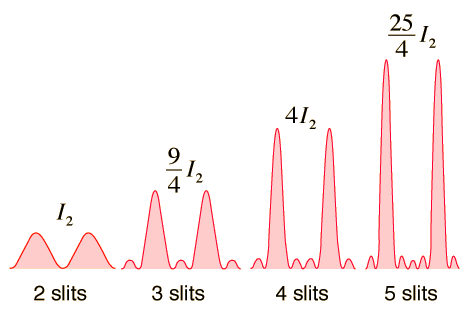
\includegraphics[width=0.5\textwidth]{figures/grating_intensity_curves.png}
\caption{The intensity curves for gratings with varying numbers of slits. Increasing the slits improves the resolution by sharpening the intensity curves.}
\label{fig:grating-intensity}
\end{figure}

The peaks have a phase difference of $\delta$ = 2m$\pi$. The closest minimums occur $\frac{\pi}{2}$ away from the peak, which occurs for a phase change of: 
\begin{equation}
\Delta \delta = \frac{2\pi}{N}
\end{equation}
Where N is the number of slits.

\begin{figure}[H]
\centering
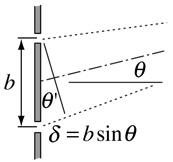
\includegraphics[width=0.5\textwidth]{figures/grating-set-up.png}
\caption{A two-slit grating showing the parameters b, $\theta$, and $\delta$}
\label{fig:grating-set-up}
\end{figure}

From the figure, 
\begin{equation}
\delta = \frac{2\pi}{\lambda}b\sin{\theta}
\end{equation}
The differential of the above is: 
\begin{equation}
d\delta = \frac{2\pi}{\lambda}b\cos{\theta}d\theta
\end{equation}
The maximum condition is:
\begin{equation}
b\sin{\theta} = m\lambda
\end{equation}
With the differential:
\begin{equation}
b\cos{\theta}d\theta = md\lambda
\end{equation}
Substituting both differentials gives:
\begin{equation}
\frac{2\pi}{N} = \frac{2\pi}{\lambda}md\lambda
\end{equation}
This simplifies to the final resolving power formula \cite{Hyperphysics}:
\begin{equation}
\boxed{R = \frac{\lambda}{\Delta \lambda} = mN}
\end{equation}

Where:
\begin{itemize}[label={}]
    \item $\lambda$ is the wavelength of interest.
    \item $\Delta \lambda$ is the resolution.
    \item $m$ is the diffraction order
\end{itemize}

\end{document}
